%importe
\documentclass{article}
\usepackage[T1]{fontenc}
\usepackage[utf8]{inputenc}
\usepackage[a4paper,top=3.5cm,left=3cm,right=3cm,bottom=2.5cm]{geometry}
\usepackage[brazil]{babel}
\usepackage{graphicx}
\usepackage{hyperref}
\usepackage{fancyhdr}
\usepackage{background}
\usepackage[a4paper,top=3.5cm,left=3cm,right=3cm,bottom=2.5cm]{geometry}
\usepackage{lmodern}

%Configurando a path das imagens
\graphicspath{{../../imagens/capitulo3/}}


%Configurando a imagem de background
\backgroundsetup{
scale=1,
angle=0,
opacity=0.4,
contents={
  
\includegraphics[width=\paperwidth,height=\paperheight]{wallpaper.png}
  }
}

%configurando os hyperlinks
\hypersetup{
    colorlinks=true,
    linkcolor=blue,
    filecolor=magenta,      
    urlcolor=cyan,
}


%configurando os headers
\pagestyle{fancy}
\fancyhf{}
\rhead{LDO}
\lhead{Capítulo 1}
\rfoot{Página \thepage}

%configurando identação e separação de parágrafos
\parindent 1.27cm
\parskip   6pt

\flushbottom

%títulos,autor e data
\title{\textbf{Capítulo 3 \\ Como é feito esse aprendizado de máquina}}
\author{Homenique Vieira Martins}
\date{Novembro de 2020}



\begin{document}
    
    %Inserindo o título
    \maketitle

    %Aumentando o tamanho padrão das fontes
    \Large

     %Iniciando a seção 'O que é'
    \section{O que é?}
    \paragraph{}Nos dias de hoje é difícil conhecer uma pessoa que nunca tenha ouvimdp falar de Machine 
    Learning, que muitas das vezes é tratado com algo magico ou de outro mundo que uma máquina 
    possa aprender principalmente com a mística que muitas empresas fazem com esse termo da moda. Porém não é bem assim, igual a um ser humano e necessário ensinar uma máquina aprenderem para que elas possam fazer coisas incríveis, e para isso existe estratégia diferentes para ensinar máquina e assim ela possa do resultado melhores para dada situação. Bora lá conhecer uma poucas dos 3 tipos de aprendizado mais populares 

    % 01 - Aprendizado Supervisionado 
    \section{Aprendizado Supervisionado:}
    \begin{figure}[ht]
        \centering
        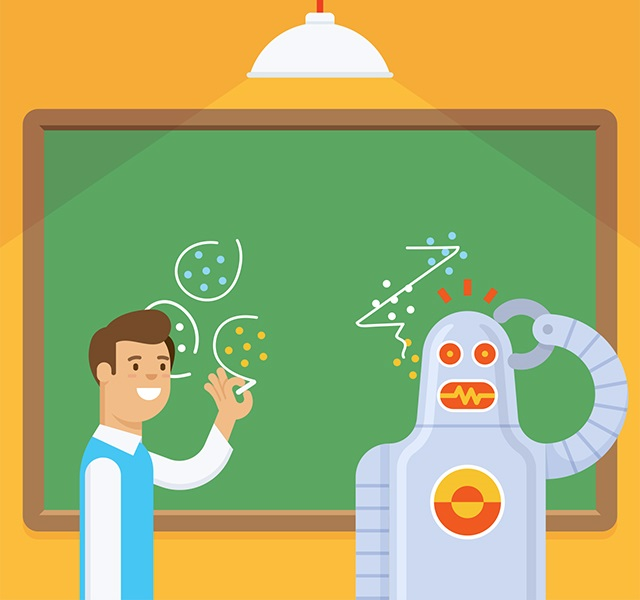
\includegraphics[scale=0.3]{robo_aprendedo.jpg}
    \end{figure}
    \paragraph{}Vamos dizer que você quer que uma maquina aprenda a reconhecer o que é um gato, para isso você
    precisa mostrar para maquina varias fotos do que é um gato e o que não é um gato, depois de uma
    certo tempo essa maquina vai começar a reconhecer gatos, porém ainda podendo errar , esse estilo
    de abordagem é conhecida como aprendizado supervisionado. Onde você informar para máquina um dado, informação, foto e etc. E junto a essa informação você também rotula a mesma para a máquina entender qual é o objeto que ela está estudado.  
    Essa abordagem é excelente para situações onde existem um padrão conhecido e você quer a máquina 
    reconheça e possa atuar em cima disso.


   % 02 - Aprendizado não Supervisionado 
    \section{Aprendizado não Supervisionado:}
    \paragraph{} Agora você não quer rotular nada, mas quer a máquina diferencie por si só o que ela encontra
    e separe em grupo que ela acha que seja parecido, isso é um aprendizado não supervisionado.
    Onde a máquina só tem o objeto, porém ela tem que classificar cada objeto a partir de um
    conjunto de variáveis  que ela acha que sejam parecidas. 
    \\
      \begin{figure}[ht]
        \centering
        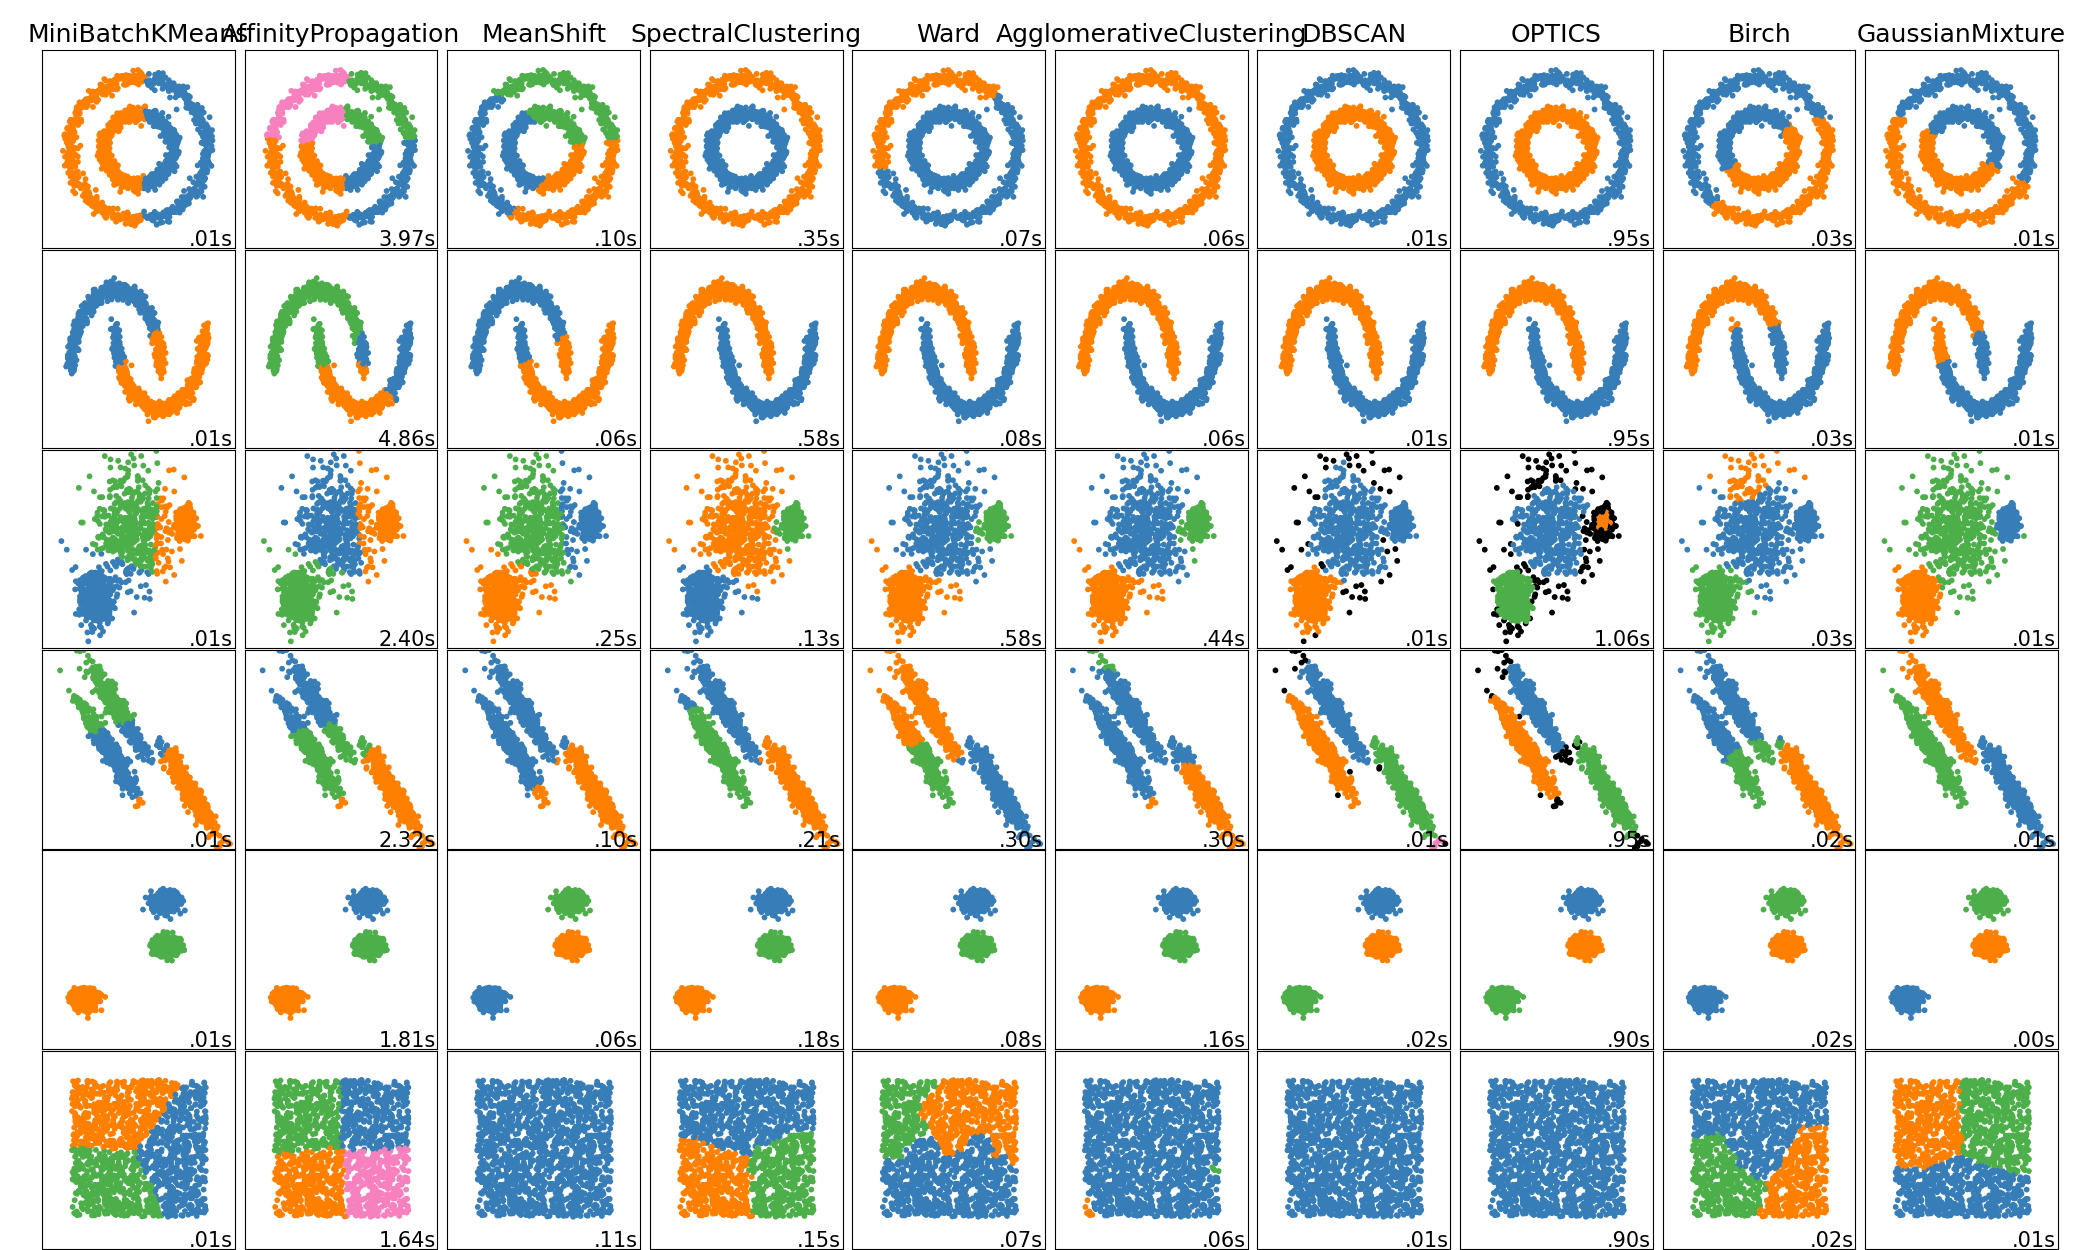
\includegraphics[scale = 0.3]{classificação de grupos.png}
    \end{figure}
    \\
    Pegamos por exemplo a Amazon,
    ela tem vários clientes com gostos diferentes, mas o que ela pode recomendar para cada cliente
    ou qual é a melhor tipo de abordagem para determinado tipo de clientes. Esse tipo de análise,
    pode ser muito bem feito por esse tipo de abordagem de aprendizado   

  % 03 - Aprendizagem por reforço
    \section{Por reforço:}
    \begin{figure}[ht]
        \centering
        
\includegraphics[scale = 0.2]{jack-jack-num-num-cookie_orig.png}
    \end{figure}

    \paragraph{}Aprendizagem por reforço é uma área de aprendizagem de máquina que investiga como agentes de software devem agir em determinados ambientes de modo a maximizar alguma noção de recompensa cumulativa.

   % 04 - Sessão Extra  
    \section*{Extra}
    Quer ver mais um pouco sobre o Machine Learning?
    \begin{itemize}
        \item\href{https://www.youtube.com/watch?v=R9OHn5ZF4Uo&t}{How Machine Learn(Com legendas em pt-br)}
        \item\href{https://www.youtube.com/watch?v=mhe5e2B9bL8&t}{Machine Learning: como ensinar uma máquina a aprender | Nerdologia Tech}
        \item\href{https://www.youtube.com/watch?v=r8KWciNmEGw}{(Aprendizado por reforço)Inteligência Artificial ESTACIONANDO carros!} 
        \item\href{https://blog.wittel.com/o-que-e-machine-learning/}{O que é machine learning e quais são as suas aplicações no mercado?}
    \end{itemize}

    \clearpage
    %Bibliografia
    \begin{thebibliography}{2}
    
    \bibitem{Nerdologia}
    Atila Lamarino \\
    \href{https://www.youtube.com/watch?v=mhe5e2B9bL8&t}{Machine Learning: como ensinar uma máquina a aprender | Nerdologia Tech}

    \bibitem{CGP}
    CGP Grey \\
    \href{https://www.youtube.com/watch?v=R9OHn5ZF4Uo&t}{How Machine Learn(Com legendas em pt-br)}

    \end{thebibliography}    
\end{document}